\documentclass[11pt]{article}
\usepackage[T1]{fontenc}
\usepackage{lmodern}
\usepackage[utf8]{inputenc}
\usepackage[margin=1in]{geometry}
\usepackage{amsmath,amssymb,amsthm}
\usepackage{graphicx,booktabs,xcolor,array}
\usepackage{listings}
\usepackage[section]{placeins}
\usepackage[hidelinks]{hyperref}
\emergencystretch=3em
\lstset{basicstyle=\ttfamily\scriptsize,breaklines=true,columns=fullflexible,frame=single,framerule=0.3pt,rulecolor=\color{gray},upquote=false}
\lstset{literate={²}{{$^2$}}1 {³}{{$^3$}}1 {·}{{$\cdot$}}1 {Γ}{{$\Gamma$}}1 {ν}{{$\nu$}}1 {π}{{$\pi$}}1 {ε}{{$\varepsilon$}}1 {₀}{{$_0$}}1 {₁}{{$_1$}}1 {₂}{{$_2$}}1 {ₖ}{{$_k$}}1 {ℂ}{{$\mathbb{C}$}}1 {ℝ}{{$\mathbb{R}$}}1 {ℕ}{{$\mathbb{N}$}}1 {←}{{$\leftarrow$}}1 {↔}{{$\leftrightarrow$}}1 {→}{{$\rightarrow$}}1 {−}{{-}}1 {≠}{{$\neq$}}1 {≤}{{$\le$}}1 {⟨}{{$\langle$}}1 {⟩}{{$\rangle$}}1 {§}{{\S}}1 {½}{{$\frac12$}}1 {⁴}{{$^4$}}1 {⁵}{{$^5$}}1 {⁷}{{$^7$}}1 {⁸}{{$^8$}}1 {⁺}{{$^+$}}1 {⁻}{{$^-$}}1 {¹}{{$^1$}}1 {⊕}{{$\oplus$}}1 {∧}{{$\wedge$}}1 {∑}{{$\sum$}}1 {–}{{-}}1 {•}{{$\bullet$}}1 {ι}{{$\iota$}}1 {ᴴ}{{$^H$}}1 {∈}{{$\in$}}1 {⊢}{{$\vdash$}}1 {∀}{{$\forall$}}1}

\newtheorem{theorem}{Theorem}[section]
\newtheorem{proposition}[theorem]{Proposition}
\newtheorem{corollary}[theorem]{Corollary}
\newtheorem{lemma}[theorem]{Lemma}
\theoremstyle{definition}
\newtheorem{definition}[theorem]{Definition}
\newtheorem{statement}[theorem]{Measured statement}
\newcommand{\grade}[1]{\textsf{\small[#1]}}
\newcommand{\Tr}{\operatorname{Tr}}
\newcommand{\Rea}{\operatorname{Re}}
\newcommand{\Ima}{\operatorname{Im}}
\newcommand{\rank}{\operatorname{rank}}
\newcommand{\sn}{\operatorname{sn}}
\title{The Weight Between and the Exit Line\\[4pt]\large Cross-block bounds for the boundary census, and where opened matter leaves the disk}
\author{Jeromie Beasley}
\date{4 November 2026}
\begin{document}
\maketitle

\noindent\emph{Prepared with AI assistance (Claude, Anthropic; and OpenAI tools for parts of the formal development). The ideas and research direction are the author's. Computation, drafting, formal checking and typesetting were done with AI tools, and every number is produced by a script printed in Appendix~B.}

\begin{abstract}
Cut a fermionic system into a region $A$ and its complement $B$. The one-body correlation matrix $C$ then has a cross block, and $X_A=C_{AB}C_{BA}$ is the weight between the two sides. We prove that $X_A$ is positive and bounded by $\tfrac14$. It is two-sided: $X_A$ and $X_B$ share their positive spectrum. It is stable in operator norm with a certified margin. It lies below the local defect $C_A-C_A^2$, and equals it on a pure state. Four times its trace bounds the Gaussian mutual information from below, with a sharp constant and no upper constant without a spectral margin. The signed boundary offset $\tau=\log\det(I-C_A)/\det C_A$ moves no faster than $\dot\tau^2\le4gS$. Two preparations with the same census, offset, cross weight and coupling saturate this bound in opposite directions.

On the PT-symmetric Su--Schrieffer--Heeger chain the correlation matrix is a biorthogonal idempotent. There the radial census survives and positivity does not. The band-averaged Petermann factor equals $2$ exactly on the line $E(0)E(\pi)=u^2$, equivalently $(w^2-v^2)^2=2u^2(w^2+v^2)$.

We construct an operator $T_R=\tfrac12\{X+\tfrac12,H\}_R$ that commutes exactly with the half-chain correlation block. The proof uses only $H(k)^2=E(k)^2I$, so it holds without Hermiticity. On its eigenvectors the entanglement levels form a ladder $\varepsilon_j=j\Delta+i\theta$. The spacing is $\Delta=2\pi K'(k)/K(k)$, with modulus $k=v'/w'$ taken from the Hermitian band hidden in the opened one. The single shared phase is $\theta=\pi F(\arcsin s\,|\,k)/K(k)$, with $s=uw/(w^2-v'^2)$. We prove that a ladder of this form crosses the unit circle of the Cayley chart all at once, and that its phase reaches $\pi/2$ exactly on the Petermann line. Both directions are proved, the converse through an explicit factorisation. The ladder form and the phase formula are verified at 200 random parameter points: commutation to $8\times10^{-12}$, spacing to $2\times10^{-8}$, phase to $4\times10^{-7}$, and the inside/outside verdict 200 of 200. They are proved in the dimer limit. Deriving them analytically from the commuting operator is the one step left open, and it is stated as such.
\end{abstract}

\paragraph{Grades.} \grade{T} proved here; \grade{L} also checked in Lean in the author's formal suite; \grade{V} verified numerically with the stated controls; \grade{R} a known result in this coordinate; \grade{C} open.

\section{Introduction}
Every finite record of a cut has two readings. One is unsigned: it counts how many boundary levels are partially occupied. The other is signed: it says which way each level leans. Both readings live on one chart,
\[
\Gamma=\frac{z-1}{z+1}=\tanh\frac{\varepsilon}{2}=1-2\nu,\qquad z=\frac{1-\nu}{\nu}=e^{\varepsilon},
\]
for an occupation $\nu$ of the region's correlation matrix. The census is the gauge without its sign. The offset is the clock face. This paper proves two things about this chart.

The first is about the \emph{weight between} the two sides of a cut, the cross block $X_A=C_{AB}C_{BA}$. Section~\ref{sec:weight} proves its order, size, symmetry, stability and information bounds. It also gives exact examples marking where the one-body record stops speaking, and proves the speed limit of the signed offset.

The second is about where \emph{opened} matter leaves the disk. Opening means a non-Hermitian generator. On the PT-symmetric dimerized chain the levels leave $|\Gamma|<1$ inside the gapped phase, before the critical point. Measured on finite blocks, that exit sits on the line $E(0)E(\pi)=u^2$, where the band-averaged Petermann factor equals $2$ (Section~\ref{sec:opened}), and the question is why it happens there. Section~\ref{sec:ladder} gives the mechanism. An operator commutes exactly with the half-chain block, and its eigenvectors organise the levels into a ladder with one shared phase. A ladder with one phase crosses the rim all at once, and its phase reaches a quarter turn exactly on the Petermann line. The exact commutation, the simultaneous crossing, the location of the crossing and a closed dimer case are proved. The ladder form and the elliptic phase formula are measured at 200 random points. Deriving them analytically is the remaining step.

\section{The chart}\label{sec:chart}
\begin{proposition}[the bridge]\label{prop:bridge}
$\Gamma=\tanh(\varepsilon/2)=1-2\nu$, and $\nu(1-\nu)=(1-\Gamma^2)/4$. The window $\nu\in[\delta,1-\delta]$ is the disk $|\Gamma|\le1-2\delta$. \grade{T}\grade{L}
\end{proposition}
\begin{proof}
$z-1=(1-2\nu)/\nu$ and $z+1=1/\nu$; $(e^\varepsilon-1)/(e^\varepsilon+1)=\tanh(\varepsilon/2)$; $1-(1-2\nu)^2=4\nu(1-\nu)$.
\end{proof}
Summed over the levels of the region, the rapidity is the signed offset
\begin{equation}\label{eq:offset}
\tau=\sum_\nu\varepsilon_\nu=\Tr[\log(I-C)-\log C]=\log\frac{\det(I-C)}{\det C},
\end{equation}
which for a number-conserving Gaussian state is $\log P(N_A=0)/P(N_A=|A|)$. The reduced state is a product over the eigenmodes of $C$, so $P(0)=\prod(1-\nu)$ and $P(|A|)=\prod\nu$ \grade{T}. The census counts levels with $\nu(1-\nu)$ above a threshold, and is blind to the sign of $\Gamma$. For example, $\mathrm{diag}(0.2,0.8)$ and $\mathrm{diag}(0.2,0.2)$ have the same defect $C-C^2=0.16I$ and offsets $0$ and $\log16$.

\begin{theorem}[the Cayley domain]\label{thm:cayley}
For $z\ne-1$, $|z+1|^2-|z-1|^2=4\Rea z$, so $|\Gamma|<1\iff\Rea z>0$ and $|\Gamma|=1\iff\Rea z=0$. For $z=e^W$, $|\tanh(W/2)|<1\iff\cos(\Ima W)>0$; on the principal branch this is $|\Ima W|<\pi/2$. \grade{T}
\end{theorem}
\begin{proof}
Expand the moduli; $\Rea e^W=e^{\Rea W}\cos\Ima W$.
\end{proof}
The real cases are checked in Lean: a positive ratio lands strictly inside, a negative ratio $S/(-s)$ with $S>s>0$ lands outside at rim distance $2s/(S-s)$, and $z=-1$ is the pole. A complex ratio does not by itself leave the disk: $z=1-i\gamma$ has $|\Gamma|^2=\gamma^2/(4+\gamma^2)<1$. Leaving needs the real part of the ratio to change sign. In the rapidity this is a quarter turn of the phase.

\section{The weight between}\label{sec:weight}
Let $C=C^*$ with $0\le C\le I$ on $\mathcal H_A\oplus\mathcal H_B$, of dimensions $a,b$, and write
\[
C=\begin{pmatrix}A_C&B_C\\B_C^*&D_C\end{pmatrix},\quad F_A=A_C-A_C^2,\quad T_A=(C-C^2)_{AA},\quad X_A=B_CB_C^*,\quad X_B=B_C^*B_C.
\]
Fix $0<\varepsilon<\tfrac12$ and put $\vartheta=\varepsilon(1-\varepsilon)$. The \emph{raw census} is $N^{\mathrm{raw}}_\varepsilon=\rank\mathbf 1_{[\varepsilon,1-\varepsilon]}(A_C)$. The \emph{boundary census} is $N^\partial_\varepsilon=\rank\mathbf 1_{[\vartheta,\infty)}(X_A)$. Counts include multiplicity and equality at the threshold.

\begin{theorem}[the weight between]\label{thm:weight}
For every such $C$:
\begin{enumerate}
\item (defect split) $F_A=T_A+X_A$; with $C^2=C$, $X_A=A_C-A_C^2$, and this needs no Hermiticity. \grade{T}\grade{L}
\item (order and size) $0\le X_A\le F_A\le\tfrac14I$, $0\le T_A\le F_A$, $\|B_C\|\le\tfrac12$, attained by $C=\tfrac12\begin{pmatrix}1&1\\1&1\end{pmatrix}$. \grade{T}\grade{L}
\item (two-sided) $X_A$ and $X_B$ have the same positive eigenvalues with multiplicity. So $N^\partial_\varepsilon(A)=N^\partial_\varepsilon(B)\le\rank B_C\le\min(a,b)$, and $\Tr X_A=\Tr X_B=\|B_C\|_F^2\le\tfrac14\min(a,b)$. \grade{T}
\item (comparison and recovery) $N^\partial_\varepsilon\le N^{\mathrm{raw}}_\varepsilon$, with equality when $C^2=C$. \grade{T}
\item (trace) $\vartheta N^\partial_\varepsilon\le\Tr X_A=\sum_{i\in A,j\in B}|C_{ij}|^2$, and $\Tr X_A=0\iff B_C=0$. \grade{T}\grade{L}
\item (local unitaries) Conjugation by $U_A\oplus U_B$ leaves every census, spectrum and trace above unchanged. \grade{T}
\end{enumerate}
\end{theorem}
\begin{proof}
(1) $(C^2)_{AA}=A_C^2+B_CB_C^*$.

(2) Compression preserves order. $C-C^2\ge0$ by the spectral theorem, hence $T_A\ge0$. Then (1) gives the two comparisons, and $F_A=\tfrac14I-(A_C-\tfrac12)^2\le\tfrac14I$, so $\|B_C\|^2=\|X_A\|\le\tfrac14$.

(3) If $B_CB_C^*u=\lambda u$ with $\lambda>0$, then $B_C^*u\ne0$ is an eigenvector of $B_C^*B_C$ with eigenvalue $\lambda$. The inverse map is $B_C/\lambda$, so the multiplicities agree.

(4) $\nu(1-\nu)-\vartheta=(\nu-\varepsilon)(1-\varepsilon-\nu)$, so $\rank\mathbf 1_{[\vartheta,\infty)}(F_A)=N^{\mathrm{raw}}_\varepsilon$. By min--max, $\lambda_j(X_A)\le\lambda_j(F_A)$. If $C^2=C$ then $T_A=0$.

(5) Each counted eigenvalue contributes at least $\vartheta$ to the trace.

(6) Block multiplication.
\end{proof}

\paragraph{The boundary coordinate.} Each eigenvalue $\lambda\in[0,\tfrac14]$ of $X_A$ has the radius $\Gamma_b=\sqrt{1-4\lambda}\in[0,1]$. On a pure state $\lambda=\nu(1-\nu)$, so $\Gamma_b=|1-2\nu|$: the boundary coordinate is the modulus of the census point and forgets its sign \grade{T}\grade{L}. For mixed states $X_A$ need not commute with $A_C$, and only the order comparisons remain.

\begin{theorem}[stability with a certified count]\label{thm:stab}
Let $C,\tilde C$ be positive contractions on the same partition, with $\delta=\|C-\tilde C\|$. Then $\|X_A(C)-X_A(\tilde C)\|\le\delta$. With $\mathcal N_Y(s)=\rank\mathbf 1_{[s,\infty)}(Y)$, for $\delta<\vartheta$,
\[
\mathcal N_{X_A(C)}(\vartheta+\delta)\le N^\partial_\varepsilon(\tilde C)\le\mathcal N_{X_A(C)}(\vartheta-\delta).
\]
If $\mathrm{dist}(\vartheta,\mathrm{spec}\,X_A(C))>\delta$ the two counts are equal. \grade{T}
\end{theorem}
\begin{proof}
$\|BB^*-\tilde B\tilde B^*\|\le(\|B\|+\|\tilde B\|)\|B-\tilde B\|\le\delta$ by Theorem~\ref{thm:weight}(2). Then apply Weyl's inequality.
\end{proof}

\begin{theorem}[near-projector comparison]\label{thm:nearproj}
With $\eta=\|C-C^2\|$, $X_A\le F_A\le X_A+\eta I$. Hence $\mathcal N_{F_A}(\vartheta+\eta)\le N^\partial_\varepsilon\le N^{\mathrm{raw}}_\varepsilon$. \grade{T}
\end{theorem}
\begin{proof}
$0\le C-C^2\le\eta I$ compresses to $0\le T_A\le\eta I$. Then use (1) and ordered-eigenvalue monotonicity.
\end{proof}

\begin{proposition}[the coordinate is Hölder]\label{prop:holder}
$|\Gamma_b(\lambda)-\Gamma_b(\tilde\lambda)|\le2\sqrt{|\lambda-\tilde\lambda|}$. If both radii are at least $g>0$, the bound is $(2/g)|\lambda-\tilde\lambda|$. The eigenvalue step does not transfer to nonnormal matrices: $\begin{pmatrix}0&1\\0&0\end{pmatrix}$ and $\begin{pmatrix}0&1\\\delta&0\end{pmatrix}$ differ by $\delta$, while their eigenvalues move by $\sqrt\delta$. \grade{T}
\end{proposition}
\begin{proof}
$|\sqrt x-\sqrt y|\le\sqrt{|x-y|}$; rationalise for the second bound.
\end{proof}

\paragraph{What the one-body record cannot say.}
\begin{proposition}[same local block, different weight between]\label{prop:extension}
Every positive contraction $A$ has the projector extension $P_A=\begin{pmatrix}A&\sqrt{A-A^2}\\\sqrt{A-A^2}&I-A\end{pmatrix}$, with $X_A(P_A)=A-A^2$. The disconnected $A\oplus(I-A)$ has the same local block and $X_A=0$. \grade{T}
\end{proposition}
\begin{proof}
The square root commutes with $A$. Multiplying the blocks gives $P_A^2=P_A=P_A^*$.
\end{proof}
Three more exact cases mark the edge of the record \grade{T}:
\begin{itemize}
\item $C=pI$ has full raw census and zero boundary census.
\item $\tfrac12(|10\rangle\langle10|+|01\rangle\langle01|)$ has $C=\tfrac12I_2$ and $X_A=0$, yet covariance $-\tfrac14$ and mutual information $\log2$.
\item $(|1100\rangle+|0011\rangle)/\sqrt2$ split $\{1,2\}|\{3,4\}$ has $X_A=0$ and entanglement entropy $\log2$.
\end{itemize}
The census reads correlation faithfully inside the quasi-free class, and only there.

\begin{proposition}[number covariance]\label{prop:var}
For a gauge-invariant quasi-free state, $\mathrm{Var}(N_A)=\Tr F_A$ and $\mathrm{Cov}(N_A,N_B)=-\Tr X_A$. On a pure Slater state, $\mathrm{Var}(N_A)=\Tr X_A$. \grade{T}
\end{proposition}
\begin{proof}
By Wick's theorem, $\mathrm{Cov}(n_i,n_j)=\delta_{ij}C_{ii}-|C_{ij}|^2$. Sum over $A\times A$ and over $A\times B$.
\end{proof}

\begin{theorem}[the weight between bounds the information across the cut]\label{thm:info}
For the same states, with $h(x)=-x\log x-(1-x)\log(1-x)$ and $I_G=\Tr h(A_C)+\Tr h(D_C)-\Tr h(C)$:
\[
4\Tr X_A\le I_G(A:B),
\]
and the constant is sharp. If $\delta I\le C\le(1-\delta)I$, then $I_G\le\Tr X_A/(\delta(1-\delta))$. Without such a margin there is no upper constant. \grade{T}
\end{theorem}
\begin{proof}
Let $S=I_A\oplus(-I_B)$ and $C_0=\tfrac12(C+SCS)=A_C\oplus D_C$. Trace Jensen states that for concave $f$, $\Tr f(\tfrac12(H+K))\ge\tfrac12\Tr f(H)+\tfrac12\Tr f(K)$. To prove it, diagonalise the mean in a basis $u_i$, then use scalar concavity and $f(\langle u,Hu\rangle)\ge\langle u,f(H)u\rangle$.

Apply it to $f=h+2x^2$, which has $f''=4-1/(x(1-x))\le0$. With unitary invariance under $S$, this gives $I_G\ge2(\Tr C^2-\Tr C_0^2)=4\Tr X_A$. On $[\delta,1-\delta]$ the function $h+x^2/(2\delta(1-\delta))$ is convex, and the same argument gives the upper bound.

Sharpness: $C=\tfrac12I+r\sigma_x$ has $I_G=4r^2+O(r^4)$ and $\Tr X_A=r^2$. For the failure without a margin, pure states with an occupation tending to $0$ have $I_G/\Tr X_A$ unbounded.
\end{proof}

\begin{theorem}[the offset speed limit]\label{thm:speed}
Let $P(t)$ be a smooth family of orthogonal projectors and $E$ an isometry onto the region. Set $C=E^\dagger PE$ with $0<C<I$, $g=\tfrac12\|\dot P\|_F^2$ and $S=\Tr[(C(I-C))^{-1}]$. Then $\dot\tau^2\le4gS$, with equality iff $\dot P\propto[P,[P,F]]$, where $F=EWE^\dagger$ and $W=-(C(I-C))^{-1}$. For $\dot P=-i[H,P]$, $g=\|PH(1-P)\|_F^2$. \grade{T}
\end{theorem}
\begin{proof}
$\dot\tau=\Tr[W\dot C]=\Tr[F\dot P]$. Differentiating $P^2=P$ shows that $\dot P$ is block off-diagonal, so only $T=[P,[P,F]]$ pairs with it. Cauchy--Schwarz gives $\dot\tau^2\le\|T\|_F^2\|\dot P\|_F^2$. Finally, $\|T\|_F^2=2\Tr[W(I-C)WC]=2S$, because $W$ and $C$ commute. For the corollary, $[H,P]$ has two adjoint blocks.
\end{proof}

\begin{proposition}[the speed budget does not choose the future]\label{prop:joint}
Take $H=\omega\sigma_x$ and $P_\pm(0)=\tfrac12(I\pm\sigma_y)$, read through the first basis vector. Both have $\nu=\tfrac12$, $\tau=0$, $X=\tfrac14$ and $g=\omega^2$. Then $\tau_\pm(t)=\mp2\operatorname{artanh}(\sin2\omega t)$: both saturate $\dot\tau^2=4gS$ at all times, in opposite directions. \grade{T}\grade{V}
\end{proposition}
\begin{proof}
The Bloch vector $(0,\pm1,0)$ rotates in the $y$--$z$ plane at rate $2\omega$. With $s=\sin2\omega t$, $S=4/(1-s^2)$ and $\dot\tau^2=16\omega^2/(1-s^2)=4gS$.
\end{proof}
The cross weight of a fixed cut is not the generator coupling of the moving projector. At $t=0$, $2\sqrt{\Tr X\cdot S}=2$ while $|\dot\tau|=4\omega$. Script \texttt{s16} checks the saturation to $5.9\times10^{-15}$. It also checks every inequality of this section on 400 random contractions and 64 interior covariances. All bounds hold, the sharp ratio runs $4.00027$, $4.0000027$, $4.00000002$, and the pure-state recovery holds to $6.8\times10^{-16}$ \grade{V}.

\section{Opened matter}\label{sec:opened}
Take the PT-symmetric SSH chain, cells $c\in\mathbb Z$, two sites $a,b$ per cell:
\[
h(k)=\begin{pmatrix}iu&v+we^{-ik}\\ v+we^{ik}&-iu\end{pmatrix},\qquad E(k)^2=v^2+w^2-u^2+2vw\cos k,
\]
with $u,v,w>0$, $v<w$, and the gap condition $E(\pi)^2=(w-v)^2-u^2>0$. In real space $H$ has $\pm iu$ on the $a$ and $b$ sites, $v$ inside a cell and $w$ from $(c,b)$ to $(c+1,a)$. Then $H^T=H$, but $H^\dagger\ne H$. Fill the lower band with the biorthogonal projector $P(k)=\tfrac12(I-h(k)/E(k))$, $E>0$, and let $C_R$ be its block on the half-chain $c\ge0$.

\begin{theorem}[what survives opening]\label{thm:open}
For any idempotent $C=\begin{pmatrix}A&B\\E&D\end{pmatrix}$, $Y_A=BE=A-A^2$, and its eigenvalues are $\nu_j(1-\nu_j)$ with algebraic multiplicity. So the radial census $\#\{|1-2\nu_j|\le r\}$ survives for every $r$. Positivity does not: $\begin{pmatrix}2&1\\-2&-1\end{pmatrix}$ is idempotent with $Y_A=-2$. \grade{T}\grade{L}
\end{theorem}
\begin{proof}
The $AA$ block of $C^2=C$ gives the first identity. Triangularising $A$ gives the eigenvalues.
\end{proof}

\begin{proposition}[the Petermann line]\label{prop:petermann}
The band projectors have $K(k)=\Tr P^\dagger P=1+u^2/E(k)^2$. The band average is
\[
\langle K\rangle=1+\frac{u^2}{E(0)E(\pi)},
\]
so $\langle K\rangle=2$ iff $E(0)E(\pi)=u^2$, iff
\begin{equation}\label{eq:exitline}
(w^2-v^2)^2=2u^2(w^2+v^2).
\end{equation}
\grade{T}\grade{L}
\end{proposition}
\begin{proof}
$\Tr P^\dagger P=\tfrac12(1+\sum|d_j|^2/|E|^2)$ for $h=d\cdot\sigma$. Here $\sum|d_j|^2=|v+we^{ik}|^2+u^2$ and $|E|^2=|v+we^{ik}|^2-u^2$. The average is $\frac1{2\pi}\int dk/(A+B\cos k)=(A^2-B^2)^{-1/2}$ with $A^2-B^2=E(0)^2E(\pi)^2$. Squaring $E(0)^2E(\pi)^2=u^4$ gives $((v+w)^2-u^2)((w-v)^2-u^2)=u^4$, that is $(w^2-v^2)^2-2u^2(w^2+v^2)=0$.
\end{proof}
At $w=1$, \eqref{eq:exitline} reads $u_{\mathrm{exit}}=(1-v^2)/\sqrt{2(1+v^2)}$. At $u=0.5$ this gives $v_{\mathrm{exit}}=0.4682$. Predicted from $\langle K\rangle=2$ before the run, the exits at $u=0.25$, $0.45$, $0.65$ are $v=0.7474014$, $0.5291503$, $0.2357262$. The measured census exits of a 40-cell block are $0.7474015$, $0.5291503$, $0.2357262$, differences $4\times10^{-8}$ and below \grade{V} (script \texttt{s05b}). The measurement uses whole-cell blocks and an endpoint filter that discards levels with $\nu$ within $10^{-9}$ of $0$ or $1$. Why the census leaves there is the question the next section answers.

\section{The exit ladder}\label{sec:ladder}
\subsection{The Hermitian band inside the opened one}
\begin{lemma}\label{lem:band}
Put $E_0=E(0)$, $E_\pi=E(\pi)$, $w'=\tfrac12(E_0+E_\pi)$, $v'=\tfrac12(E_0-E_\pi)$. Then $v'^2+w'^2=v^2+w^2-u^2$, $v'w'=vw$ and
\[
E(k)^2=|v'+w'e^{ik}|^2,
\]
the band of a Hermitian dimerized chain with hoppings $v'<w'$. Its modulus is $k=v'/w'$, and $k'=\sqrt{1-k^2}=\sqrt{E_0E_\pi}/w'$. \grade{T}
\end{lemma}
\begin{proof}
$E_0^2+E_\pi^2=2(v^2+w^2-u^2)$ and $E_0^2-E_\pi^2=4vw$. Then $v'^2+w'^2=\tfrac12(E_0^2+E_\pi^2)$, $v'w'=\tfrac14(E_0^2-E_\pi^2)$ and $w'^2-v'^2=E_0E_\pi$.
\end{proof}

\subsection{An operator that commutes with the half-chain block}
Let $X$ be the cell-position operator, $X_{(c,\alpha),(c',\beta)}=c\,\delta_{cc'}\delta_{\alpha\beta}$.
\begin{theorem}[the commuting operator]\label{thm:commute}
Let $T=\tfrac12\{X+\tfrac12,H\}$. Then $[P,T]=0$, and $T=T_L\oplus T_R$ has no entries across the cut between cells $-1$ and $0$. Consequently
\[
[C_R,T_R]=0,
\]
entrywise, as an identity of infinite matrices. $T_R$ is tridiagonal, with
\begin{gather*}
T_R\big|_{(c,a),(c,a)}=iu(c+\tfrac12),\qquad T_R\big|_{(c,b),(c,b)}=-iu(c+\tfrac12),\\
T_R\big|_{(c,a),(c,b)}=v(c+\tfrac12),\qquad T_R\big|_{(c,b),(c+1,a)}=w(c+1),
\end{gather*}
and it is symmetric. \grade{T}
\end{theorem}
\begin{proof}
The gap condition gives $E(k)^2\ge E_\pi^2>0$, so $P(k)$ is analytic and periodic. The real-space entries $P_{cc'}=\frac1{2\pi}\int e^{ik(c-c')}P(k)\,dk$ therefore decay exponentially, and every product below is an absolutely convergent sum. Integration by parts gives $[X,P]_{cc'}=(c-c')P_{cc'}=\frac{i}{2\pi}\int e^{ik(c-c')}\partial_kP(k)\,dk$. Since $[P,H]=0$,
\[
[P,\{X,H\}]=\{[P,X],H\}\;\longleftrightarrow\;-i\{\partial_kP,h\}=\tfrac i2\{\partial_k(h/E),h\}.
\]
Differentiating $(h/E)^2=I$ gives $\{\partial_k(h/E),h/E\}=0$, so the right side vanishes. The shift by $\tfrac12$ commutes with $P$ trivially, so $[P,T]=0$.

The entry $T_{ij}=\tfrac12(x_i+x_j+1)H_{ij}$ crosses the cut only for $i=(-1,b)$, $j=(0,a)$, where $x_i+x_j+1=0$. So $T=T_L\oplus T_R$. Then $(PT)_{RR}=C_RT_R+P_{RL}T_{LR}=C_RT_R$ and $(TP)_{RR}=T_RC_R$. The listed entries follow from those of $H$.
\end{proof}
The construction is that of Peschel and of Eisler and Peschel for Hermitian chains~\cite{peschel03,peschel04,eislerpeschel13,eislerpeschel17}. What is new here is that it uses only $h(k)^2=E(k)^2I$. That relation survives the non-Hermitian opening, so the commuting operator survives with it. Since $C_R$ is bounded and $T_R$ is banded, $C_R$ maps each eigenspace of $T_R$ into itself. A simple eigenvector of $T_R$ is therefore an eigenvector of $C_R$, and the levels of $C_R$ can be indexed by those of $T_R$.

\subsection{The ladder}
\begin{statement}[the edge ladder]\label{st:ladder}
Let $K=K(k)$ and $K'=K(k')$ be the complete elliptic integrals of the first kind for the modulus of Lemma~\ref{lem:band}. Put
\[
s=\frac{uw}{w^2-v'^2}\in(0,1),\qquad \theta=\frac{\pi}{K}\,F(\arcsin s\,|\,k)\in(0,\pi),\qquad \Delta=\frac{2\pi K'}{K}.
\]
Equivalently, $\sn(\theta K/\pi\,|\,k)=s$. Then the levels of $C_R$ on the eigenvectors of $T_R$ localised at the cut are
\[
\varepsilon_j=\log\frac{1-\nu_j}{\nu_j}=j\Delta+i\theta,\qquad j\in\mathbb Z.
\]
All levels share one phase, and there is no real offset. \grade{V}
\end{statement}
\noindent\emph{Evidence} (script \texttt{s15}). The test uses 200 random points with $w=1$, $v\in(0.02,0.7)$, $u\in(0.02,0.9)$ and gap $E_\pi\ge0.2$, of which 16 lie past the exit line. The block has 90 cells, inside a $6000$-momentum chain. Results:
\begin{itemize}
\item the eigen-residual of $C_R$ on the edge eigenvectors of $T_R$ is at most $8.4\times10^{-12}$;
\item the relative spacing error is at most $1.7\times10^{-8}$;
\item the phase error is at most $4.2\times10^{-7}$ on the levels $j=0,\pm1$;
\item the domain condition $s<1$ holds, with maximum $0.913$ at the test points and $1-4\times10^{-8}$ on a $400\times400$ grid of the whole gapped region, where $s\to1$ only at the critical line.
\end{itemize}
Deeper levels have $\nu$ within $10^{-10}$ of $0$ or $1$. There the nonnormal eigenproblem is ill-conditioned, and they are not used. At $u=0$, $k=v/w$ and the spacing is the elliptic spacing of the Hermitian dimerized chain known from corner-transfer-matrix methods~\cite{peschel04,peschelEisler09}, with the protected $\nu=\tfrac12$ edge level at $j=0$ \grade{R}. Opening the chain keeps the spacing of the hidden Hermitian band and rotates the whole ladder by one phase.

\subsection{The exit theorem}
\begin{theorem}[the exit ladder]\label{thm:exit}
\begin{enumerate}
\item[(a)] (one phase, one crossing) If $\varepsilon_j=j\Delta+i\theta$ with $\theta\in(0,\pi)$, then every $\Gamma_j=\tanh(\varepsilon_j/2)$ lies on the circular arc through $-1$, $i\tan(\theta/2)$ and $1$. Either all $|\Gamma_j|<1$, or all $|\Gamma_j|=1$, or all $|\Gamma_j|>1$, according as $\theta<\pi/2$, $\theta=\pi/2$ or $\theta>\pi/2$.
\item[(b)] (the crossing is the Petermann line) For $\theta$ as in Statement~\ref{st:ladder},
\[
\theta=\frac\pi2\iff E(0)E(\pi)=u^2\iff\langle K\rangle=2\iff(w^2-v^2)^2=2u^2(w^2+v^2).
\]
Moreover $\theta<\pi/2$ on the side $E(0)E(\pi)>u^2$ and $\theta>\pi/2$ on the other.
\item[(c)] (the dimer limit, exact) At $v=0$ the half-chain block has exactly one level off $\{0,1\}$, with $\varepsilon=2i\arcsin(u/w)$. This equals the formula of Statement~\ref{st:ladder} at $v=0$. That level leaves the disk exactly at $w^2=2u^2$, which is \eqref{eq:exitline} at $v=0$.
\end{enumerate}
\grade{T}
\end{theorem}
\begin{proof}
(a) By Theorem~\ref{thm:cayley}, $|\tanh(W/2)|<1\iff\cos\Ima W>0$. Here $\Ima\varepsilon_j=\theta$ for every $j$, in the principal range. The image of the line $\{x+i\theta\}$ under $W\mapsto\tanh(W/2)$ is a circle arc. Its endpoints are $\pm1$ as $x\to\pm\infty$, and $x=0$ gives $\tanh(i\theta/2)=i\tan(\theta/2)$.

(b) On $(0,K)$, $\sn(\cdot\,|\,k)$ increases strictly from $0$ to $1$, and $\sn(K/2\,|\,k)^2=1/(1+k')$~\cite{byrd}. So $\theta=\pi/2$ iff $s^2(1+k')=1$. Put $W=w'$ and $r=\sqrt{E_0E_\pi}$, so that $k'=r/W$ (Lemma~\ref{lem:band}). Then
\[
\mathcal F:=u^2w^2(W+r)-W(w^2-v'^2)^2=0.
\]
Lemma~\ref{lem:band} makes $w^2$ and $v^2$ the roots of $x^2-(2W^2-r^2+u^2)x+W^2(W^2-r^2)=0$. With $\delta=u^2-r^2$ and $D=\sqrt{4W^2u^2+\delta^2}$, the larger root ($w>v$) is $w^2=W^2+\tfrac12(\delta+D)$, and $w^2-v'^2=\tfrac12(u^2+r^2+D)$. So $\mathcal F=\mathcal F(D)$ is a polynomial in $D$. Multiplying by its conjugate $\mathcal F(-D)$ and reducing with $D^2=4W^2u^2+\delta^2$ gives the identity
\[
\mathcal F(D)\,\mathcal F(-D)=W\,r^2u^2\,(W+r)^2\,(W-r)\,(u^2-r^2).
\]
Since $0<r<W$ and $u>0$, $\mathcal F(D)=0$ forces $u^2=r^2=E(0)E(\pi)$.

Conversely, on $u^2=r^2$ we have $\delta=0$, $D=2Wu$, $w^2=W(W+u)$ and $w^2-v'^2=u(W+u)$. Then $s^2=w^2/(W+u)^2=W/(W+u)=1/(1+k')$. The remaining equivalences are Proposition~\ref{prop:petermann}.

For the sides: $\theta$ is continuous in $(v,u)$ on the gapped region and equals $\pi/2$ only on the line. Each side of the line is connected, since for fixed $v$ it is an interval in $u$ with continuous endpoints. As $u\to0$, $s\to0$ and $\theta\to0$; at $v=0$, $\theta=2\arcsin(u/w)>\pi/2$ for $u^2>w^2/2$.

(c) At $v=0$, $H$ is a direct sum of dimers on $\{(c,b),(c+1,a)\}$ with matrix $\begin{pmatrix}-iu&w\\w&iu\end{pmatrix}$ and $E=\sqrt{w^2-u^2}$. The half-chain $c\ge0$ contains whole dimers, whose blocks are idempotent with $\nu\in\{0,1\}$, and the single site $(0,a)$ of the cut dimer. For that site, $\nu=\tfrac12(1-iu/E)$, so $z=(E+iu)/(E-iu)$ has $|z|=1$ and $\varepsilon=2i\arctan(u/E)=2i\arcsin(u/w)$. At $v=0$ we have $v'=0$, $k=0$, $K=\pi/2$ and $F(\phi\,|\,0)=\phi$, so $s=u/w$ and $\theta=2\arcsin(u/w)$. The level leaves where $2\arcsin(u/w)=\pi/2$, that is $w^2=2u^2$, and $E(0)E(\pi)=w^2-u^2=u^2$ there.
\end{proof}
Sympy confirms that $\mathcal F$ vanishes on the line, and that the product reduces to the factored form above. Script \texttt{s15} returns $|\theta-\pi/2|\le6.7\times10^{-16}$ on the line at six values of $v$, and the dimer limit to $2.2\times10^{-16}$ \grade{V}.

\begin{figure}[!htbp]\centering
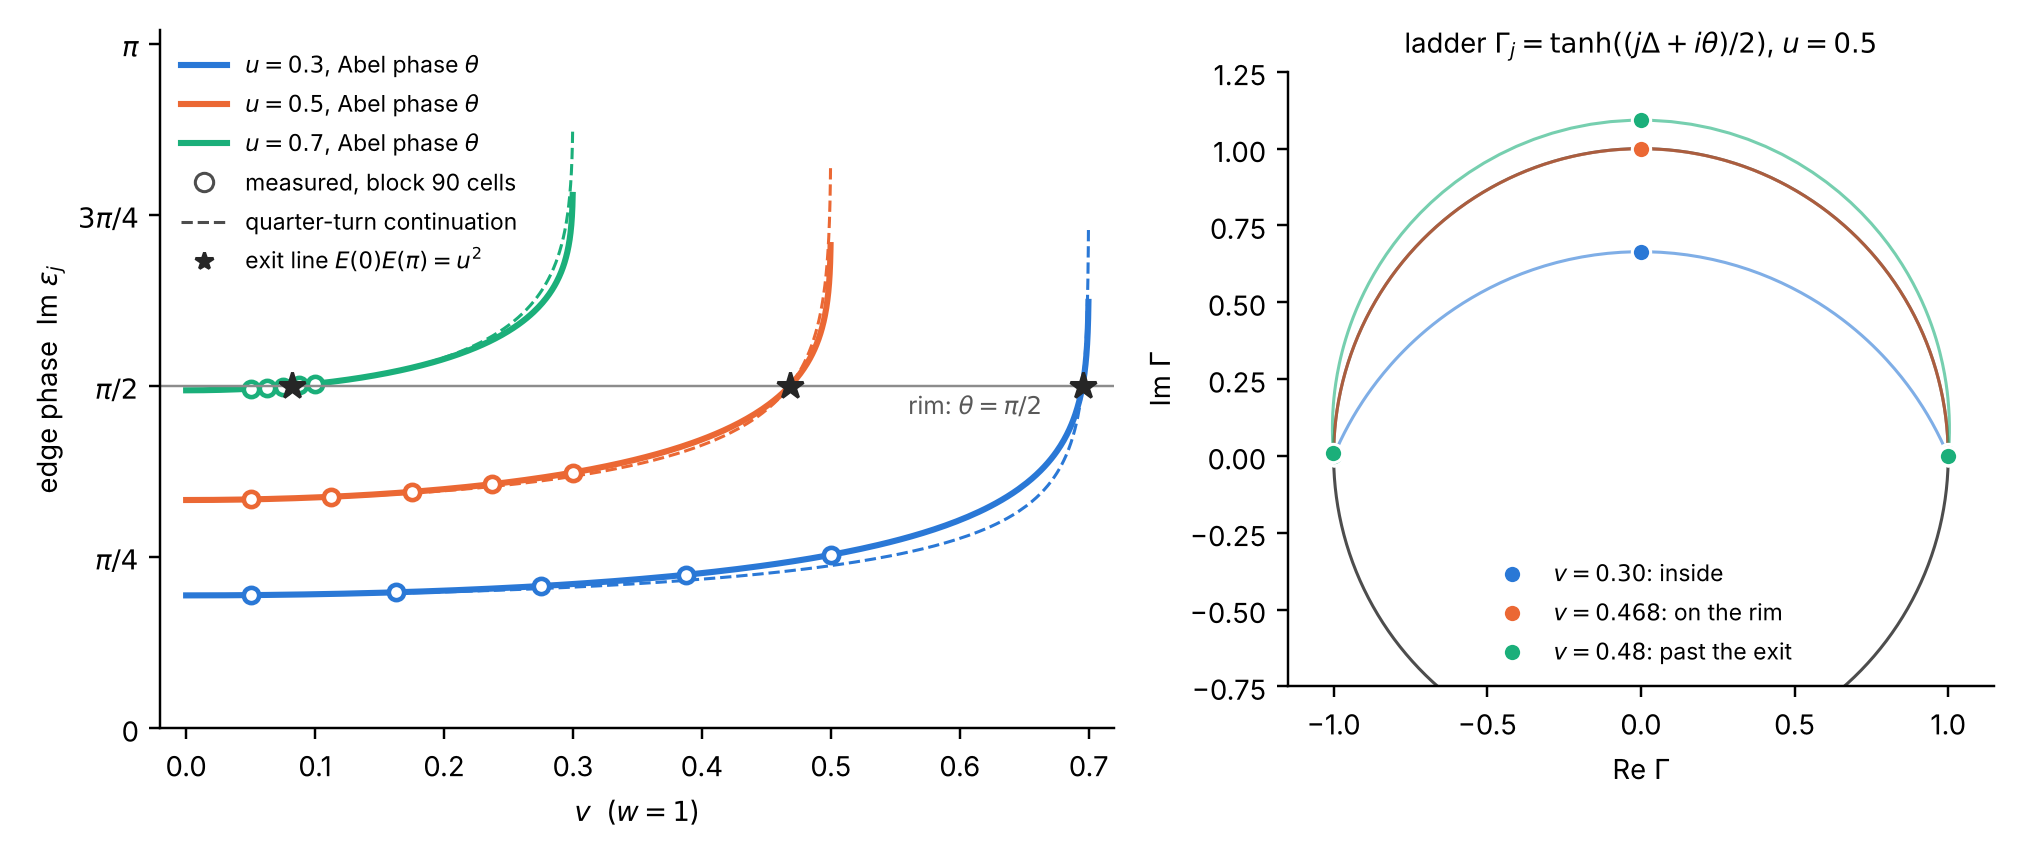
\includegraphics[width=\textwidth]{../figures/fig09_exit_ladder.png}
\caption{Left: the shared edge phase $\theta$ from Statement~\ref{st:ladder} (solid) against $v$ at three values of $u$ ($w=1$). Open circles: measured $\Ima\varepsilon_0$, block of 90 cells. Dashed: the quarter-turn continuation $2\arctan(u/\sqrt{E_0E_\pi})$. Stars: the exit line \eqref{eq:exitline}, where every solid curve crosses $\pi/2$. Right: the ladder $\Gamma_j$, $j=-3,\dots,3$, at $u=0.5$, inside, on and past the exit. Each ladder sits on one arc through $\pm1$, so it crosses the rim all at once.}
\label{fig:ladder}
\end{figure}

\subsection{What the theorem explains, and its scope}
\begin{enumerate}
\item \emph{Why the exit is filter-independent on this chain.} The levels nearest the endpoints, $\Rea\varepsilon_j\to\pm\infty$, cross with the centre level. A filter that discards them does not move the crossing until it begins to discard ill-conditioned levels it should keep. The filter audit bears this out (ring $2000$, block $40$, $v=0.5$, $w=1$). The massless exit holds at $u=0.4743416$, with $\langle K\rangle=2.000000002$, for every filter from $10^{-6}$ through $10^{-9}$. It moves only in the seventh digit at $10^{-10}$ and in the fourth at $10^{-12}$, where the filter keeps levels within $10^{-10}$ of the endpoints, whose eigenvalues are ill-conditioned \grade{V} (script \texttt{incoming\_exit\_filter}).
\item \emph{Why the quarter-turn continuation fits only at the exit.} The continued endpoint offset $\Gamma_{\mathrm{end}}=i\gamma$, $\gamma=u/\sqrt{E_0E_\pi}$, is the apex $i\tan(\theta/2)$ of the arc only at $v=0$ and on the exit line. Elsewhere $\tan(\theta/2)\ne\gamma$ (Figure~\ref{fig:ladder}, dashed). At nine points on the approach to the exit ($u=0.3,0.5,0.7$), plain finite blocks measure a census rotation above the continuation by $4\times10^{-6}$ to $3.4\times10^{-2}$, independent of block size (script \texttt{s11}). That rotation is the Abel phase: at the same nine points and blocks of $40$ and $80$ cells, the largest census rotation equals $\theta/\pi$ to $7.2\times10^{-7}$ (script \texttt{s18}). This is a check on Statement~\ref{st:ladder} that does not use the commuting operator \grade{V}.
\item \emph{Partition.} The cut runs between cells. With $w=0$ every whole-cell block is idempotent and nothing leaves, even where $\langle K\rangle=2$. That is consistent with (c): the level that exits belongs to a dimer cut in two.
\item \emph{Other bands.} Theorem~\ref{thm:commute} uses only $h(k)^2=E(k)^2I$ and nearest-cell hopping, so the commuting operator exists for any such two-band chain. Statement~\ref{st:ladder} and part (b) are stated for real $u$ only, where the on-site term is purely imaginary. The massive band $d=(t_1+\cos k,\sin k,m+i\gamma)$ has a complex on-site term. At $m=0.4$ its census exits far earlier, at $\langle K\rangle\approx1.02$ (script \texttt{s06}), and the exit moves with the filter, from $\gamma=0.2716$ at $10^{-6}$ to $0.1228$ at $10^{-12}$ (script \texttt{incoming\_exit\_filter}). Whether its ladder still carries a single phase is not tested here.
\end{enumerate}

\paragraph{The open step.} Theorem~\ref{thm:commute} fixes the eigenvectors. Theorem~\ref{thm:exit} turns any ladder of the measured form into the exit law. What remains is to derive the ladder form and the elliptic phase of Statement~\ref{st:ladder} from $T_R$ analytically. In the Hermitian case this is done by the corner transfer matrix. Here the natural route is the Wiener--Hopf factorisation of the band symbol on the elliptic curve $y^2=-z(v'+w'z)(v'z+w')$. On that curve the phase appears as the Abel image of the point $z=-v/w$, where the opened eigenvector $(E-iu,\,-(v+wz))$ degenerates. That derivation is open \grade{C}. With it, the exit law on the coupled PT-symmetric chain would be a theorem end to end.

\section{Status}\label{sec:status}
\begin{center}\small
\begin{tabular}{p{0.62\textwidth}l}\toprule
Result & Grade\\\midrule
Bridge & \grade{T}\grade{L}\\
Cayley domain (real cases also in Lean) & \grade{T}\\
Weight between: split, order, two-sidedness, comparison, trace, local unitaries & \grade{T}\grade{L}\\
Operator-norm stability, near-projector comparison, Hölder radius & \grade{T}\\
Projector extension and three exact limits of the one-body record & \grade{T}\\
$4\Tr X_A\le I_G$, sharp; upper bound with margin, none without & \grade{T}\grade{V}\\
Offset speed limit and the opposite-direction saturating pair & \grade{T}\grade{V}\\
Radial census survives opening; positivity does not & \grade{T}\grade{L}\\
Petermann line $\langle K\rangle=2\iff(w^2-v^2)^2=2u^2(w^2+v^2)$ & \grade{T}\grade{L}\\
Hidden Hermitian band; commuting operator $[C_R,T_R]=0$ & \grade{T}\\
Ladder crosses the rim all at once; its phase is $\pi/2$ exactly on the Petermann line (both directions); dimer limit & \grade{T}\\
Ladder form $\varepsilon_j=j\Delta+i\theta$, elliptic spacing and Abel phase, 200 random points & \grade{V}\\
Finite-block census exit on the line, to $4\times10^{-8}$; filter audit & \grade{V}\\
Census rotation of plain blocks equals the Abel phase, to $7.2\times10^{-7}$ & \grade{V}\\
Analytic derivation of the ladder from $T_R$ & \grade{C}\\\bottomrule
\end{tabular}
\end{center}

\begin{thebibliography}{9}
\bibitem{peschel03} I.~Peschel, Calculation of reduced density matrices from correlation functions, \emph{J. Phys. A} \textbf{36} (2003) L205.
\bibitem{peschel04} I.~Peschel, On the reduced density matrix for a chain of free electrons, \emph{J. Stat. Mech.} (2004) P06004.
\bibitem{peschelEisler09} I.~Peschel and V.~Eisler, Reduced density matrices and entanglement entropy in free lattice models, \emph{J. Phys. A} \textbf{42} (2009) 504003.
\bibitem{eislerpeschel13} V.~Eisler and I.~Peschel, Free-fermion entanglement and spheroidal functions, \emph{J. Stat. Mech.} (2013) P04028.
\bibitem{eislerpeschel17} V.~Eisler and I.~Peschel, Analytical results for the entanglement Hamiltonian of a free-fermion chain, \emph{J. Phys. A} \textbf{50} (2017) 284003.
\bibitem{byrd} P.~F.~Byrd and M.~D.~Friedman, \emph{Handbook of Elliptic Integrals for Engineers and Scientists}, 2nd ed., Springer (1971).
\end{thebibliography}

\appendix
\section{Conventions}
Logarithms are natural. $K(k)=F(\pi/2\,|\,k)$ with $F(\phi\,|\,k)=\int_0^\phi(1-k^2\sin^2t)^{-1/2}dt$ (the scripts call \texttt{mpmath} with parameter $m=k^2$). The biorthogonal projector uses the principal square root $E(k)>0$, which is valid throughout the gapped region. The cut lies between cells $-1$ and $0$, and the region is $c\ge0$; in the scripts it is the left edge of a finite block of 90 cells. The phases $\Ima\varepsilon$ use the principal logarithm.

\section{Scripts}
Each listing prints the numbers quoted in the text. The outputs are reproduced after each listing.

\subsection*{B.1 \texttt{s15\_exit\_ladder.py}}
\lstinputlisting[language=Python]{../scripts/s15_exit_ladder.py}
\lstinputlisting{../outputs/s15_exit_ladder.txt}
\subsection*{B.2 \texttt{s16\_weight\_between\_checks.py}}
\lstinputlisting[language=Python]{../scripts/s16_weight_between_checks.py}
\lstinputlisting{../outputs/s16_weight_between_checks.txt}
\subsection*{B.3 \texttt{fig09\_exit\_ladder.py}}
\lstinputlisting[language=Python]{../scripts/fig09_exit_ladder.py}
\subsection*{B.4 Symbolic check of Theorem~\ref{thm:exit}(b)}
\lstinputlisting[language=Python]{../scripts/s17_exit_converse_sympy.py}
\lstinputlisting{../outputs/s17_exit_converse_sympy.txt}
\subsection*{B.5 \texttt{s18\_census\_rotation\_vs\_abel.py}}
\lstinputlisting[language=Python]{../scripts/s18_census_rotation_vs_abel.py}
\lstinputlisting{../outputs/s18_census_rotation_vs_abel.txt}
\subsection*{B.6 \texttt{s05b\_predict\_exit.py} (with its helper \texttt{s05a\_exit\_line.py})}
\lstinputlisting[language=Python]{../scripts/s05a_exit_line.py}
\lstinputlisting[language=Python]{../scripts/s05b_predict_exit.py}
\lstinputlisting{../outputs/s05b_predict_exit_rerun_20261104.txt}
\subsection*{B.7 \texttt{s06\_second\_model\_exit\_law.py}}
\lstinputlisting[language=Python]{../scripts/s06_second_model_exit_law.py}
\lstinputlisting{../outputs/s06_second_model_exit_law_rerun_20261104.txt}
\subsection*{B.8 \texttt{s11\_exit\_quarter\_turn.py}}\noindent Its helper \texttt{nhssh\_lib\_and\_s03a\_occupations.py} comes first.
\lstinputlisting[language=Python]{../scripts/nhssh_lib_and_s03a_occupations.py}
\lstinputlisting[language=Python]{../scripts/s11_exit_quarter_turn.py}
\lstinputlisting{../outputs/s11_exit_quarter_turn_rerun_20261104.txt}
\subsection*{B.9 \texttt{incoming\_exit\_filter.py} (imported audit, prepared with OpenAI tools)}
\lstinputlisting[language=Python]{../external/gpt_formal_20261103/review/incoming_exit_filter.py}
\lstinputlisting{../outputs/incoming_exit_filter_rerun_20261104.txt}
\end{document}
